\subsection{Q10.20 data 09202021 10082021 10312021 11092021 grouped by scenario \& x_first}

\begin{comment}
                     EFPR        EO      EFNR     n    pvalue
(frauth, False)  0.475000  0.525000  0.462500  40.0  0.765738
(frauth, True)   0.513889  0.486111  0.486111  36.0  0.847316
(icu, False)     0.484848  0.515152  0.651515  33.0  0.419930
(icu, True)      0.645161  0.354839  0.580645  31.0  0.081224
(rent, False)    0.391892  0.608108  0.432432  37.0  0.115944
(rent, True)     0.500000  0.500000  0.442857  35.0  0.900056
\end{comment}

\begin{table}[h]
    \centering
    \begin{tabular}{|c|c|c|c|c|c|c|}
        \hline
        scenario & x_first & EFPR & EO & EFNR & n & p-value\\
        \hline
        frauth & False & 0.475 & \textbf{0.525} & 0.463 & 40.0 & 0.766\\
		frauth & True & \textbf{0.514} & 0.486 & 0.486 & 36.0 & 0.847\\
		icu & False & 0.485 & \textbf{0.515} & \textbf{0.652} & 33.0 & 0.420\\
		icu & True & \textbf{0.645} & 0.355 & \textbf{0.581} & 31.0 & 0.081\\
		rent & False & 0.392 & \textbf{0.608} & 0.432 & 37.0 & 0.116\\
		rent & True & 0.500 & 0.500 & 0.443 & 35.0 & 0.900\\
		
        \hline
    \end{tabular}
    \caption{Grouped by scenario x_first}
    \label{tab:my_label}
\end{table}
\begin{figure}[h]
    \centering
    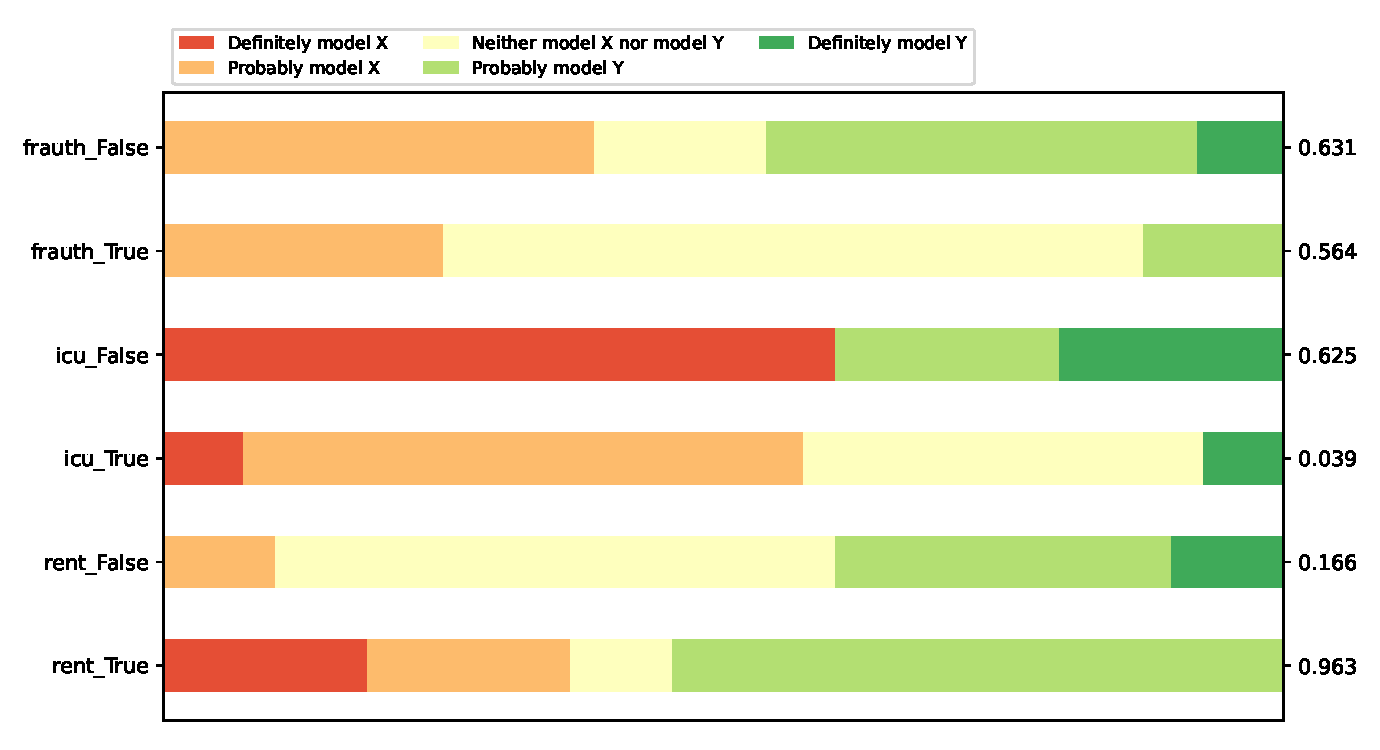
\includegraphics[width=0.8\textwidth]{figures/Q10.20/09202021_10082021_10312021_11092021/Q10.20_scenario_x_first.pdf}
    \caption{Grouped by scenario \& x_first}
    \label{fig:my_label}
\end{figure}
